% Copyright 2019 Clara Eleonore Pavillet

% Author: Clara Eleonore Pavillet
% Description: This is an unofficial Oxford University Beamer Template I made from scratch. Feel free to use it, modify it, share it.
% Version: 1.0

\documentclass{beamer}
\usepackage[utf8]{inputenc}

\usepackage{graphicx}
\title{Mathematical and Computational Modelling}
%\titlegraphic{\includegraphics[width=2cm]{Theme/Logos/OxfordLogoV1.png}}
\author{Christian Parpart, Kei Thoma}
\date{} %\today

\begin{document}

\begin{frame}
\frametitle{Problemstellung}

\begin{center}
\begin{tabular}{ c c c }
$p_0$ & $p_1$ & $p_2$ \\
\hline
172 & 93 & 120 \\
309 & 193 & 258 \\
302 & 187 & 255 \\
283 & 174 & 238 \\
443 & 291 & 317 \\
298 & 184 & 246 \\
319 & 205 & 265 \\
419 & 260 & 304 \\
361 & 212 & 292 \\
267 & 169 & 242 \\
337 & 216 & 272 \\
230 & 144 & 191
\end{tabular}
\end{center}

\end{frame}

\begin{frame}
\frametitle{Theorie}
\begin{align*}
p_0 =& a + b \cdot p_1 \\
\text{bzw.} \\
p_0 =& a + b \cdot p_1 + c \cdot p_2
\end{align*}

Wir können anhand dieser Gleichung eine Matrix aufstellen. Die wir mit der QR-Zerlegung lösen!

Wieso QR-Zerlegung? $\rightarrow$ Die Kondition kann nicht schlechter werden.

\end{frame}

\begin{frame}
\frametitle{Algorithmus: QR-Zerlegung (vom NLA Skript)}
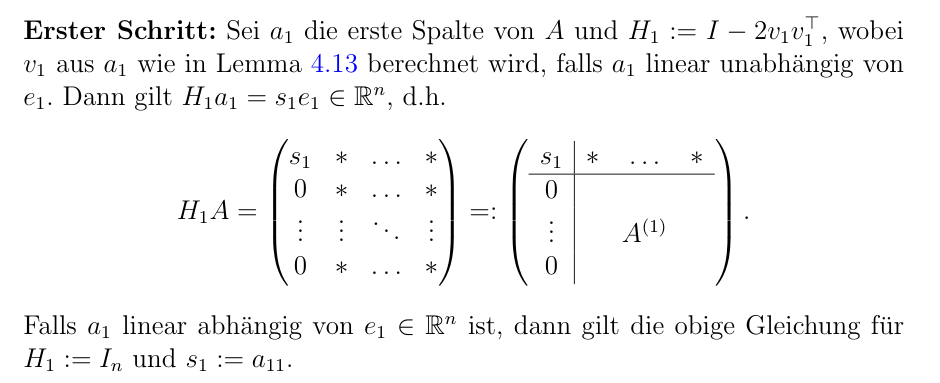
\includegraphics[width=\textwidth]{alg1.png}
\end{frame}

\begin{frame}
\frametitle{Algorithmus: QR-Zerlegung (vom NLA Skript)}
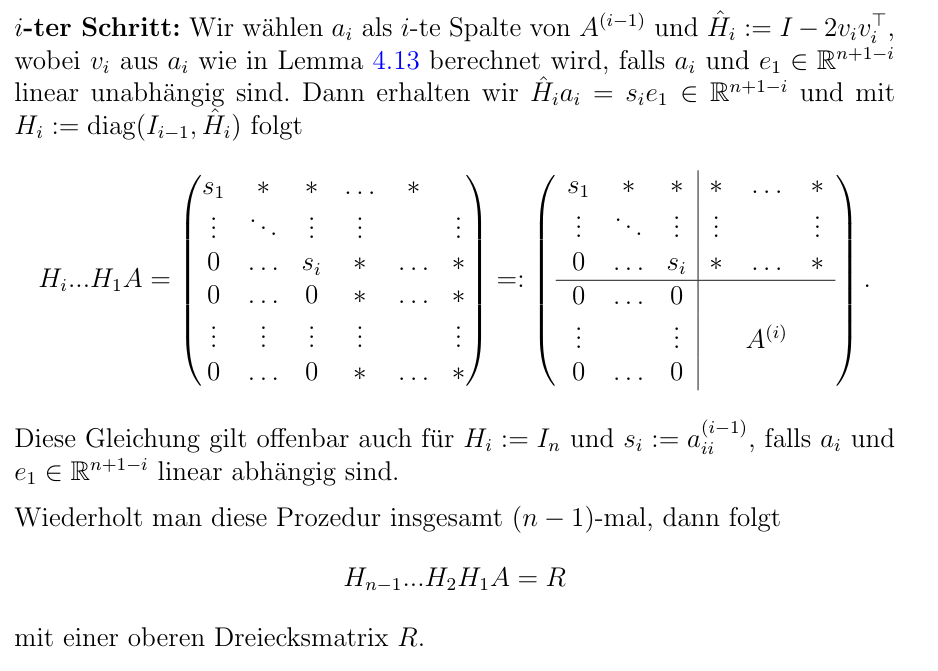
\includegraphics[width=\textwidth]{alg2.png}
\end{frame}

\begin{frame}
\frametitle{Algorithmus: QR-Zerlegung, was dann?}

Bestimme dann zuerst:

\begin{align*}
A = QR \\
\begin{pmatrix}
z_1 \\
z_2
\end{pmatrix} = Q^T b \\
R = \begin{pmatrix}
R_1 \\
0
\end{pmatrix}
\end{align*}

Dann durch Rückwärtseinsetzen $R_1 z_1$ lösen um $x$ zu bestimmen.

\end{frame}


\begin{frame}
\frametitle{Implementierung und Experimente}

Mit den ursprünglichen Daten ...

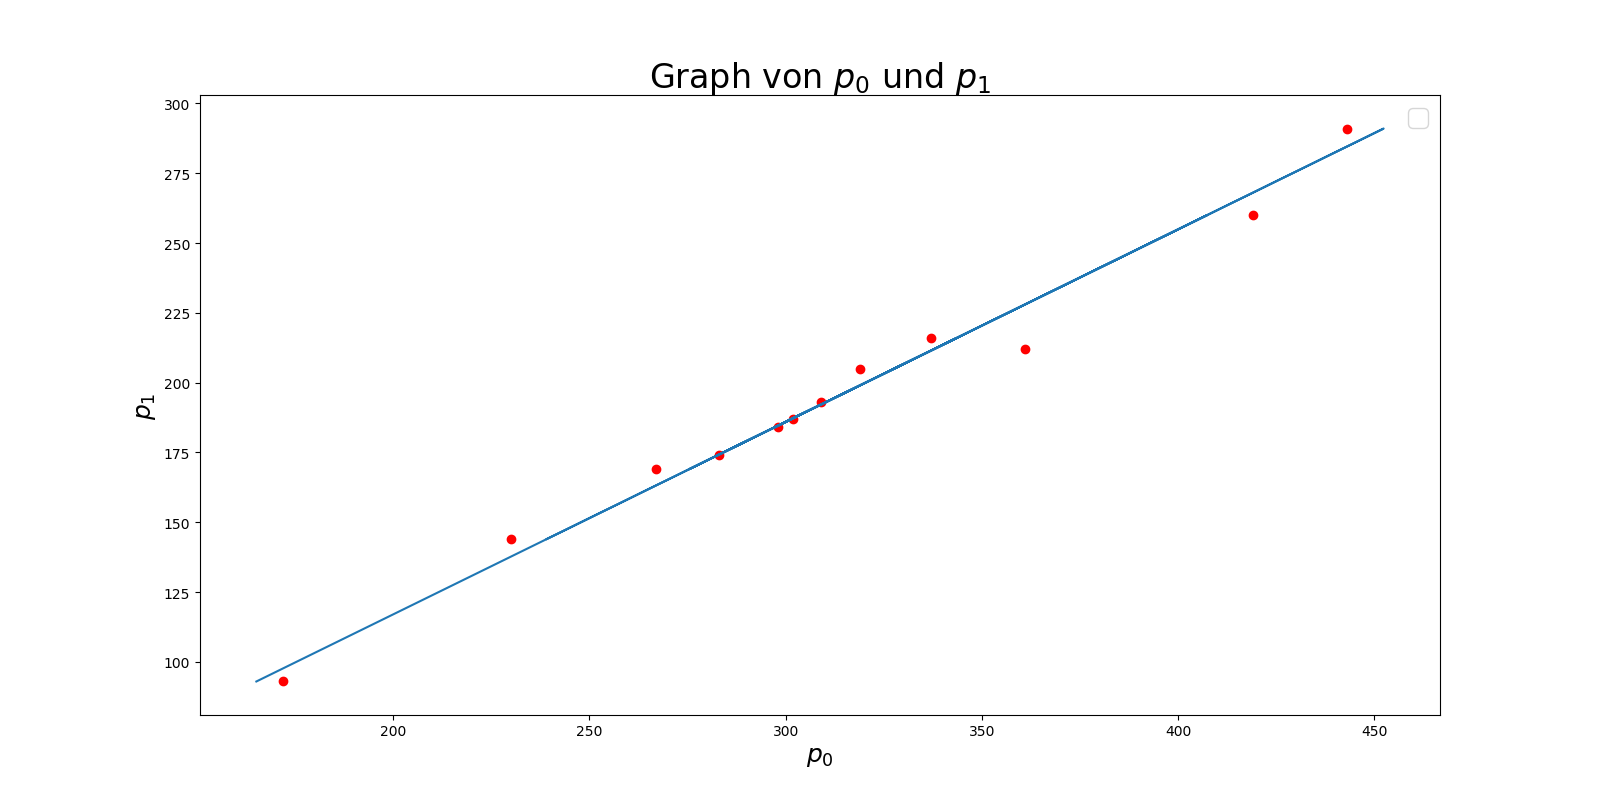
\includegraphics[width=\textwidth]{plot.png}

Kondition: $A = 74.26$, $A^T A = 5514.75$

Residuum: 32.90 (ohne $p_2$), 32.09 (mit $p_2$)
\end{frame}

\begin{frame}
Hier wurde nur die ersten 6 Werte betrachtet ...

\frametitle{Implementierung und Experimente}
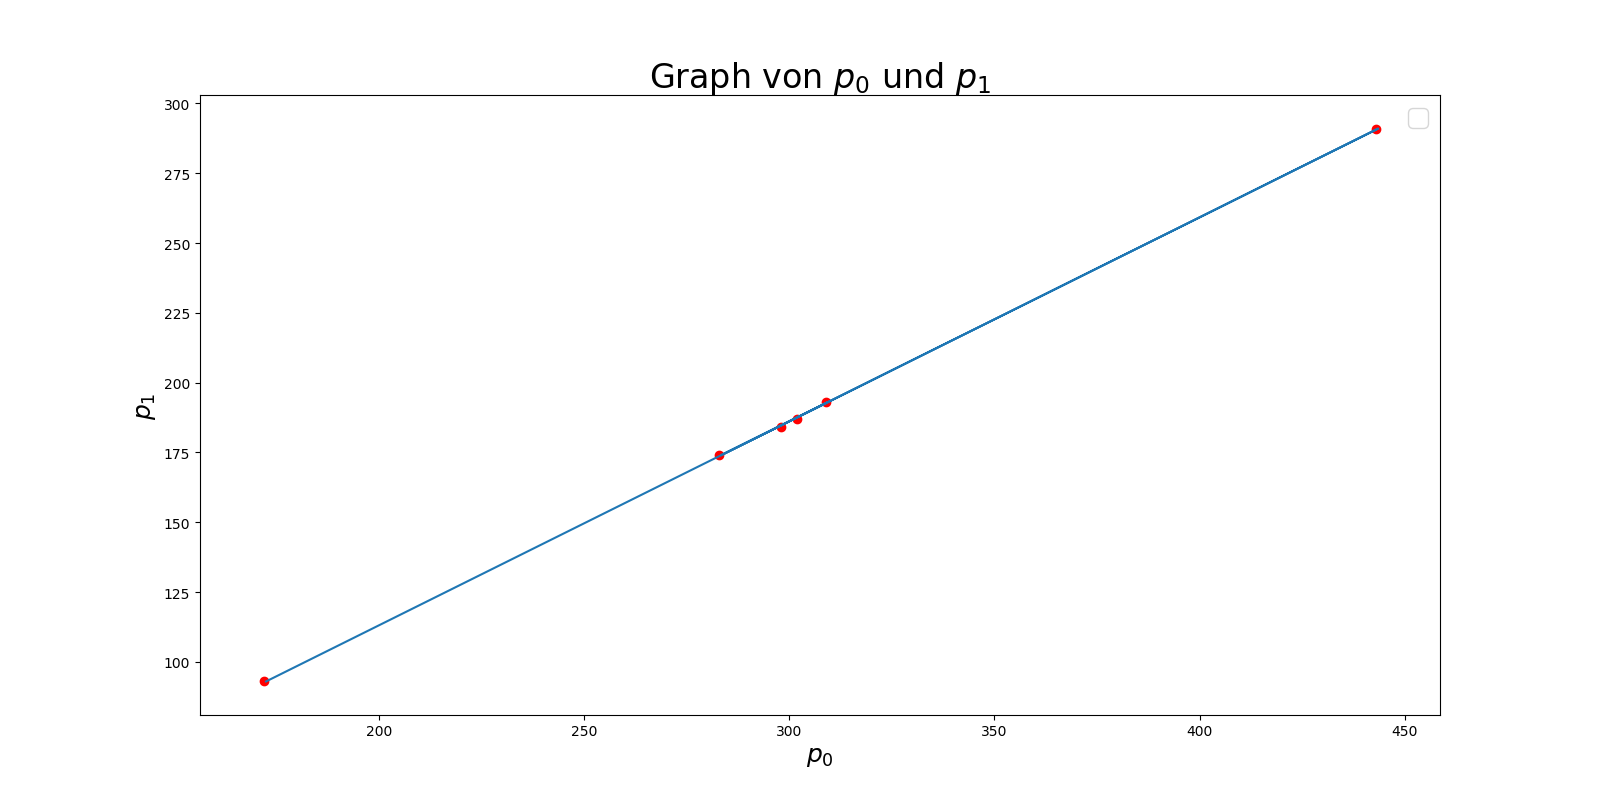
\includegraphics[width=\textwidth]{plot1.png}

Kondition: $A = 72.47$, $A^T A = 5252.05$

Residuum: 1.54 (ohne $p_2$), 1.26 (mit $p_2$)
\end{frame}

\begin{frame}
Hier wurden die Werte gerundet ...

\frametitle{Implementierung und Experimente}
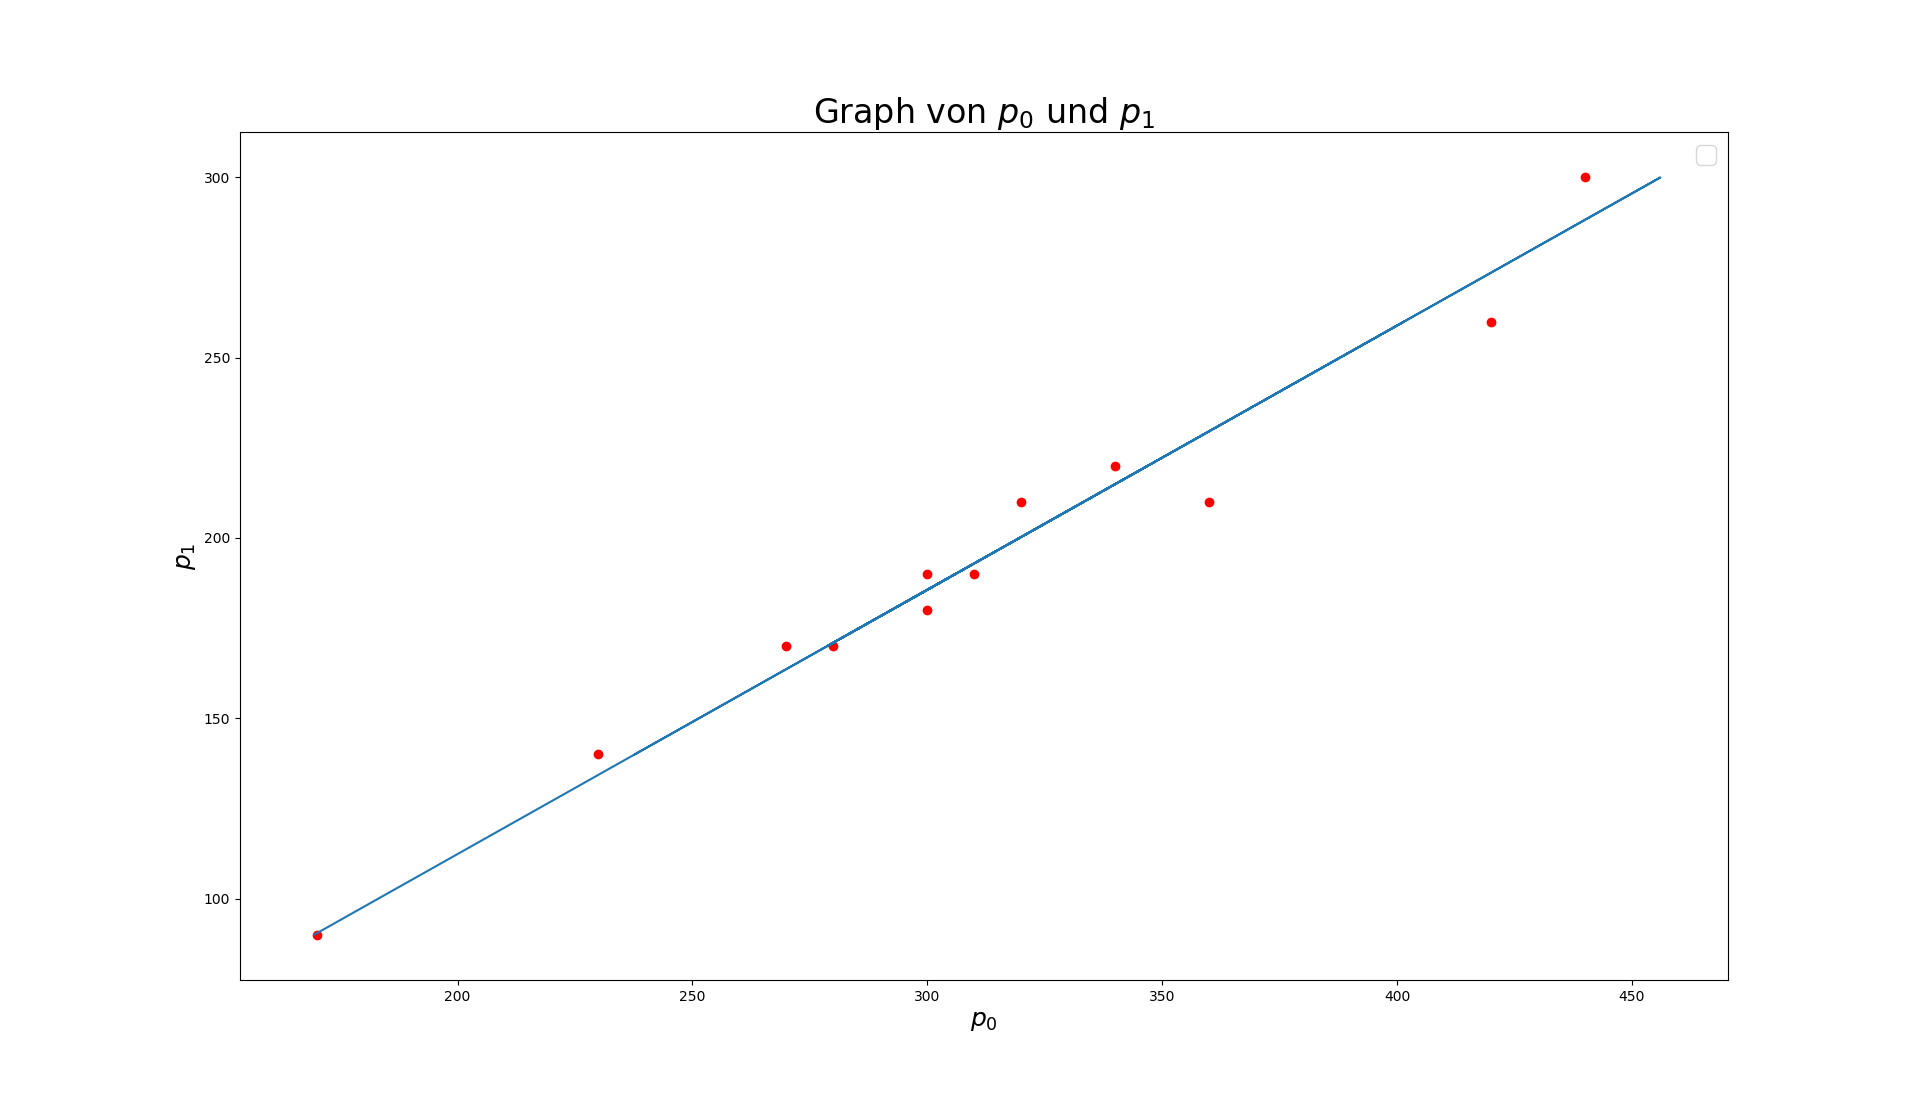
\includegraphics[width=\textwidth]{plot2.png}

Kondition: $A = 55.74$, $A^T A = 3107.40$

Residuum: 42.28 (ohne $p_2$), 39.43 (mit $p_2$)
\end{frame}


\begin{frame}
\frametitle{Auswertung und Zusammenfassung}

\begin{itemize}


\item Je weniger Werte, desto kleiner das Residuum, aber das Ergebnis wird wahrscheinlich recht inakkurat.
\item Präzisere Inputwerte sind vorzuziehen.
\end{itemize}

\end{frame}

\begin{frame}
\frametitle{Literatur}
\begin{enumerate}

\item \textit{Numerische Lineare Algebra}, Prof. Dr. Caren Tischendorf

\end{enumerate}

\end{frame}


\end{document}